
\section*{Chapitre 7 - Angles (2)}
\addcontentsline{toc}{section}{Chapitre 7 - Angles (2)}


\subsection*{I. Nature des angles et mesure}
\addcontentsline{toc}{subsection}{I. Nature des angles et mesure}



\begin{Propriétés*}[c]
\begin{minipage}[c]{0.7\textwidth}
\begin{itemize}[label=\textcolor{Couleur1}{$\bullet$}]
\item Un angle plein correspond à un tour complet. Il mesure 360°.
\item Un angle plat correspond à un demi-tour. Il mesure 180°.
\item Un angle droit correspond à un quart de tour. Il mesure 90°.
\item Un angle nul mesure 0°.
\end{itemize}
\end{minipage} \hfill
\begin{minipage}[c]{0.3\textwidth}
\begin{center}
\begin{tikzpicture}[scale=.9]
        % Secteurs colorés
    \fill[Couleur6!40] (0,0) -- (0:1.3) arc (0:45:1.3) -- cycle;
     \fill[Couleur3!85] (0,0) ++(0:1) arc (0:180:1);
    \fill[Couleur11!80] (0,0) ++(0:0.6) arc (0:360:0.6);
    \fill[Couleur8] (0,0) -- (-0.3,0) -- (-0.3,0.3) -- (0,0.3) -- cycle;
        
    % Demi-cercle de mesure
    \draw[very thick] (0,0) ++(0:2) arc (0:180:2);
    \draw[very thick] (-2.2,0) --(2.2,0);
    \draw[very thick] (0,-0.7) --(0,2.2);
    \draw[very thick] (0,0) --(1.6,1.6);
    
   
    % Étiquettes
    \node[Couleur6!60] at (1.55,0.55) {45°};
    \node[Couleur3!85] at (0.6,1.4) {180°};
    \node[Couleur11!80] at (-1.1,-0.5) {360°};
    \node[Couleur8] at (-1.3,0.55) {90°};
\end{tikzpicture}
\end{center}
\end{minipage} 

\end{Propriétés*}

\begin{Remarque}
\leavevmode\vspace{-\baselineskip}
La somme des mesures d'angles supplémentaires est donc égale à 180°.
\end{Remarque}
\vspace{0.8cm}

\begin{Propriété}[c]
Deux angles opposés par le sommet ont la même mesure.
\end{Propriété}


\subsection*{II. Construction d'angles}
\addcontentsline{toc}{subsection}{II. Construction d'angles}

\begin{Méthode} Construire un angle avec un rapporteur. \\
Construire l'angle $\widehat{TOM}$ de mesure 100°.\\
\begin{minipage}[t]{0.6\textwidth}
\vspace{0pt}
\begin{enumerate}[label=\textcolor{Couleur7}{\textbf{\arabic*.}}, leftmargin=*, itemsep=4pt]
    \item On trace [OT) ou [OM) à l'aide d'une règle.
    \item Placer le \textbf{centre} du rapporteur sur le \textbf{sommet} de l'angle (ici le point O).
    \item Aligner le \textbf{côté} de l'angle déjà tracé, avec un \textbf{0} du rapporteur (noter si c'est le 0 intérieur ou le 0 extérieur).
    \item Repérer à l'aide d'une petite marque la mesure voulue (en étant vigilant sur la graduation utilisée).
    \item Relier la marque et le sommet de l'angle.
\end{enumerate}
\end{minipage}\hfill
\begin{minipage}[t]{0.4\textwidth}



\end{minipage}

\end{Méthode}

\begin{Remarque}
Méthode en vidéo : LLS.fr/M6Methode24.
\end{Remarque}

\subsection*{III.  Bissectrice}
\addcontentsline{toc}{subsection}{III. Bissectrice}


\begin{Définition}[c]
La \textbf{bissectrice} d'un angle est la demi-droite qui partage cet angle en deux angles adjacents égaux.
\end{Définition}

\begin{Exemple}
\begin{minipage}[c]{0.6\textwidth}
\begin{enumerate}
\item Tracer [AD), la bissectrice de l'angle $\widehat{\text{BAC}}$
\item Que peut-on dire des angles $\widehat{\text{BAD}}$ et $\widehat{\text{DAC}}$ ? 

\ligne

\item Si $\widehat{\text{BAC}}=74$° , quelle est la mesure de $\widehat{\text{BAD}}$ et $\widehat{\text{DAC}} $ ?

\ligne

\ligne

\ligne

\end{enumerate}
\end{minipage} \hfill
\begin{minipage}[c]{0.4\textwidth}

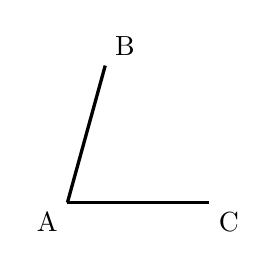
\begin{tikzpicture}[scale=0.6]
    % Points
    \coordinate (A) at (0,0);
    \coordinate (B) at (0.8,2.9);  % Angle d'environ 74° avec l'horizontale
    \coordinate (C) at (3,0);      % Horizontale (0°)

    
    % Rayons
    \draw[very thick] (A) -- (B);
    \draw[very thick] (A) -- (C);

    

    
    % Labels des points
    \node[below left] at (A) {A};
    \node[above right] at (B) {B};
    \node[below right] at (C) {C};


\end{tikzpicture}


\end{minipage} 

\end{Exemple}

